% Candidate source: src-2323f00197bbd8d5c8353a847fc0e7ccfc52169ca219272ee58990ae4b6ecba3
% Source PDF SHA-256: be2accb36a086126db90ee7c5a217e08e55429053a4167df1ad58bbfb213de46
% PDF page 1 (printed page 180), question 17.
% Redraw follows visible/hidden edges; quadrangular pyramid P-ABCD with rhombus base.
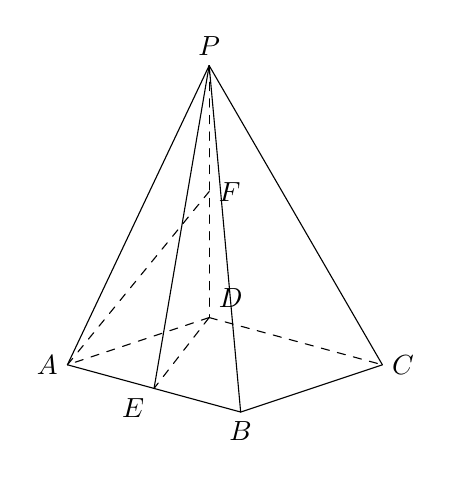
\begin{tikzpicture}[line cap=round,line join=round,>=latex,x=1.0cm,y=1.0cm]
  % Vertices
  \coordinate (D) at (0,0);
  \coordinate (P) at (0,3.2);
  \coordinate (A) at (-1.8,-0.6);
  \coordinate (C) at (2.2,-0.6);
  \coordinate (B) at (0.4,-1.2);

  % Midpoints E on AB and F on PD
  \coordinate (E) at (-0.7,-0.9);
  \coordinate (F) at (0,1.6);

  % Hidden edges
  \draw[dashed] (P) -- (D);
  \draw[dashed] (D) -- (A);
  \draw[dashed] (D) -- (C);
  \draw[dashed] (D) -- (E);
  \draw[dashed] (A) -- (F);

  % Visible edges: lateral
  \draw (P) -- (A);
  \draw (P) -- (B);
  \draw (P) -- (C);
  \draw (P) -- (E);

  % Visible edges: base
  \draw (A) -- (B) -- (C);

  % Labels
  \node[above] at (P) {$P$};
  \node[right] at (F) {$F$};
  \node[above right] at (D) {$D$};
  \node[left] at (A) {$A$};
  \node[below left] at (E) {$E$};
  \node[below] at (B) {$B$};
  \node[right] at (C) {$C$};
\end{tikzpicture}
